\chapter{OMNeT++}

\label{sec:OMNeT}
OMNeT++ represents a simulation framework written in C++ and is a open source project.
The commercial supported version is OMNEST and provides licensing models, whereas OMNeT++ is only available for academic or non-profit use.
The intention of OMNeT++ is providing infrastructure for writing simulations for various fields.
This includes an architecture for simulating different modules.
The architecture and topology of simulations is built with the different OMNeT++ components.

\section{Components}
Within an OMNeT++ simulation different components are used.
Each component is described with a \emph{network description} (NED) file.

The outermost component is a network.
A Network consists of other components like modules and channels.
The simulated topology and the connections (channels) between modules are defined within the network.

A simple module is the smallest part within a simulated OMNeT++ hierarchy and represent a functional unit.
For this functional unit the behavior for handling messages, the possible connections and additional parameters can be defined.

The possible connections of modules are represented by gates, which can be connected to a channel.
Multiple simple modules can be connected via channels and condensed to a compound module.
Such compound modules can be used in the same way as simple modules, but represent bigger functional groups.

The connections in between modules are represented by channels, which also allow custom behavior and additional parameters (e.g. delay, latency, jitter).
An example network including simple modules connected to a compound module is shown in figure \ref{fig:OMNeTComponents}.
Each module shown in figure \ref{fig:OMNeTComponents} defines two gates which can ether be an input, output or bidirectional gate.

\begin{figure}
    \centering
    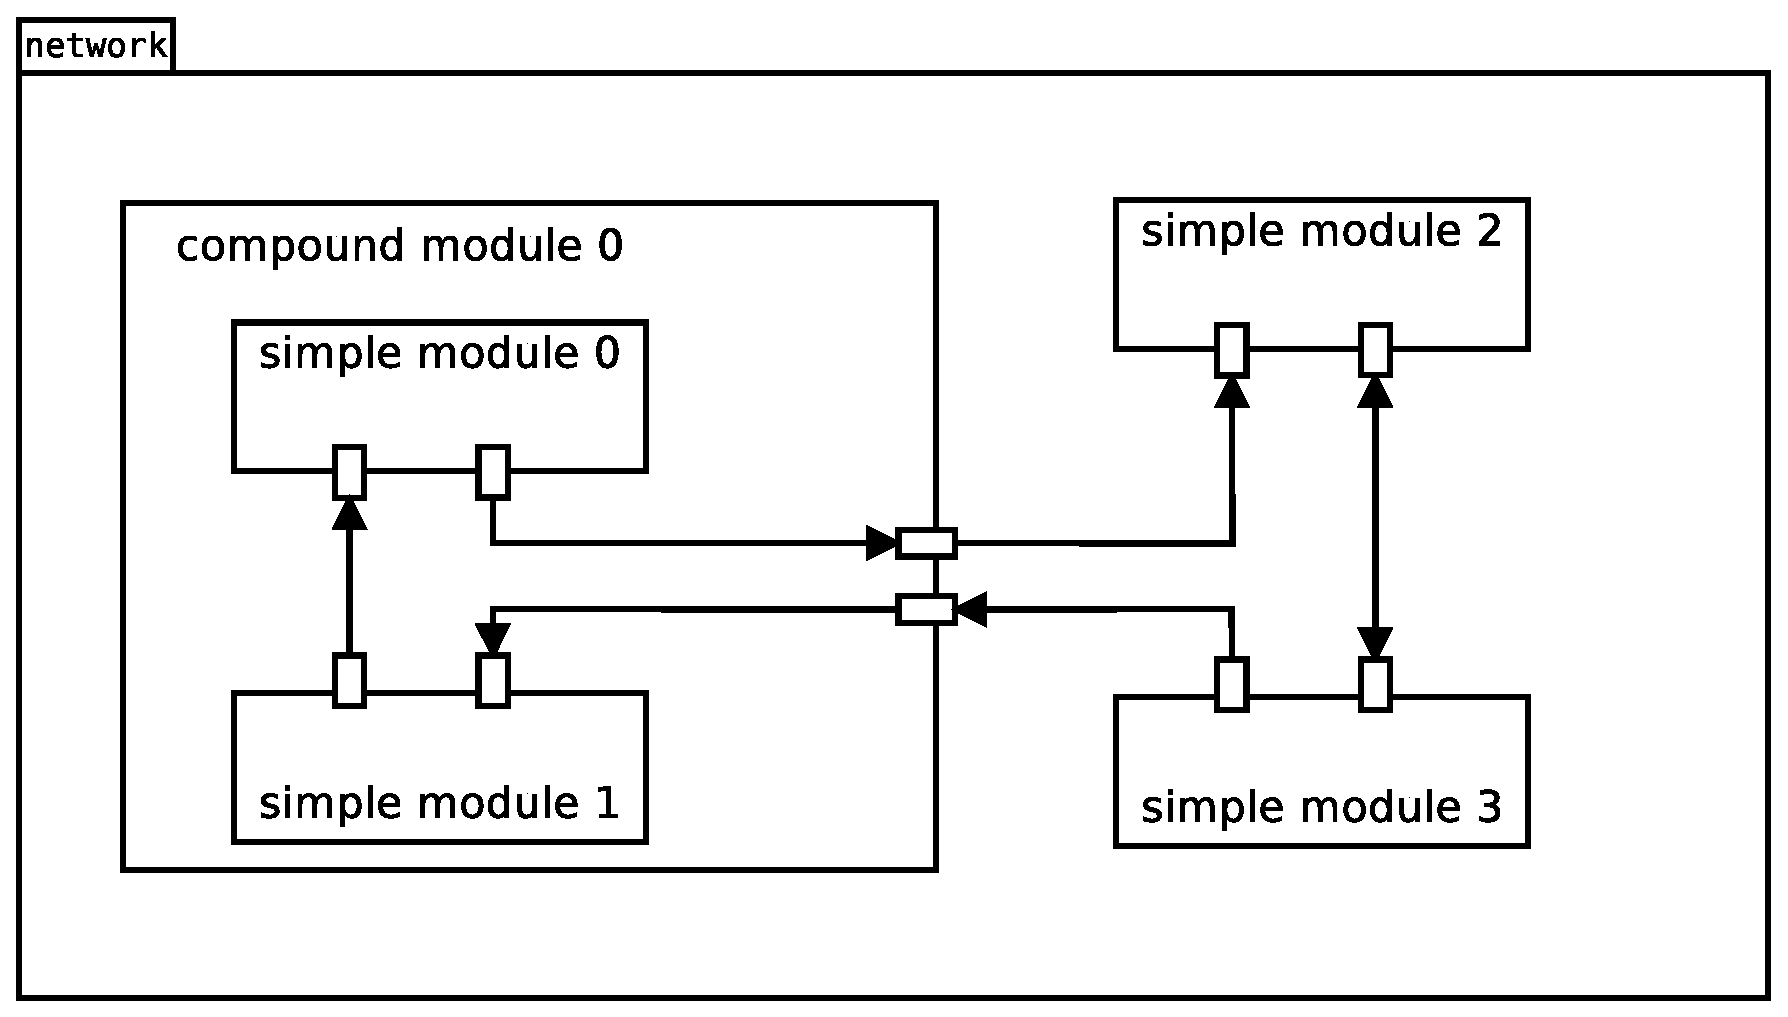
\includegraphics[width=0.9\columnwidth]{OMNeTComponents.eps}
    \caption{OMNeT++ components in an example network}
    \label{fig:OMNeTComponents}
\end{figure}

Each custom module and channel is defined in the \emph{NED} language.
Specific functionality for custom components is implemented in the according C++ code.
This assignment is usually done with identical names of the \emph{NED} file and the C++ code.
Examples and the combination of \emph{NED} files and C++ code is shown in \cite[chapter 3, chapter 4]{OMNETMANUAL}.
The components can embed any functionality implemented in C/C++.
The usage of external libraries or language features is not limited, but must be used with care due to the effect on simulation performance.


\section{Messages}
Transmitted data are encapsulated in another component called messages.
Messages are a fundamental component of a OMNeT++ simulation as they does not only transport data they can also represent functional messages like jobs, events or tasks.
The meaning behind a message is depending on the written simulation and the simulated system.

These messages can also be customized for holding a specific set of data like a protocol header, checksum, etc. or other specific data.
The existing message class \emph{cMessage} and its derived specialization \emph{cPacket} provide different members and functions which can be used for simulations.
These include control information, type information, time stamp, etc. and are included for making developing a simulation easier.
Adding a few simple datafields to a message can be ether done by subclassing \emph{cMessage} or \emph{cPacket} or using the \emph{NED} syntax.
By defining a custom message using \emph{NED} a customized subclass will be generated by the simulation and can be normally used as Message.

Any module can send a message via a connected channel for this sent message a time is defined.
This time describes the moment when the message should be sent to the channel.
The mechanism of messages is also used for implementing timeouts, timers, etc. by sending a specific message to the current module, this is a so called \emph{self-message}.
These \emph{self-message} is handled by the same function as any other message coming from other modules.
For the identification of \emph{self-messages} there is a built in function available.
More information about messages and the possibilities of customized messages are given in \cite[chapter 5]{OMNETMANUAL}.

Each message sent ether by another module or by the current module itself represents an event for the simulation with an according time, at which this event should happen, or the message should be delivered/received.
The execution and the handling of such created events is done by the simulation core and defines the execution order and the performance of the simulation.
Handling these events can be done in various ways and define the type of implemented simulation.
These simulations based on events are event based discrete simulations, the definitions of this type and the explanation of different simulation types are shown in the next section.

\section{Running an OMNeT++ simulation}
A simulation application developed with OMNeT++ can be run in different ways using different simulation environments.

\subsection{Tkenv}
OMNeT++ provides the graphical environment \emph{Tkenv} for developing simulations and demographic purposes.

\subsection{Cmdenv}